\documentclass[tikz,border=8pt]{standalone}
\usepackage{amsmath,amssymb}
\usetikzlibrary{arrows.meta,calc,decorations.pathreplacing,patterns,shapes.geometric,positioning,shadings,decorations.markings,decorations.pathmorphing}

\begin{document}
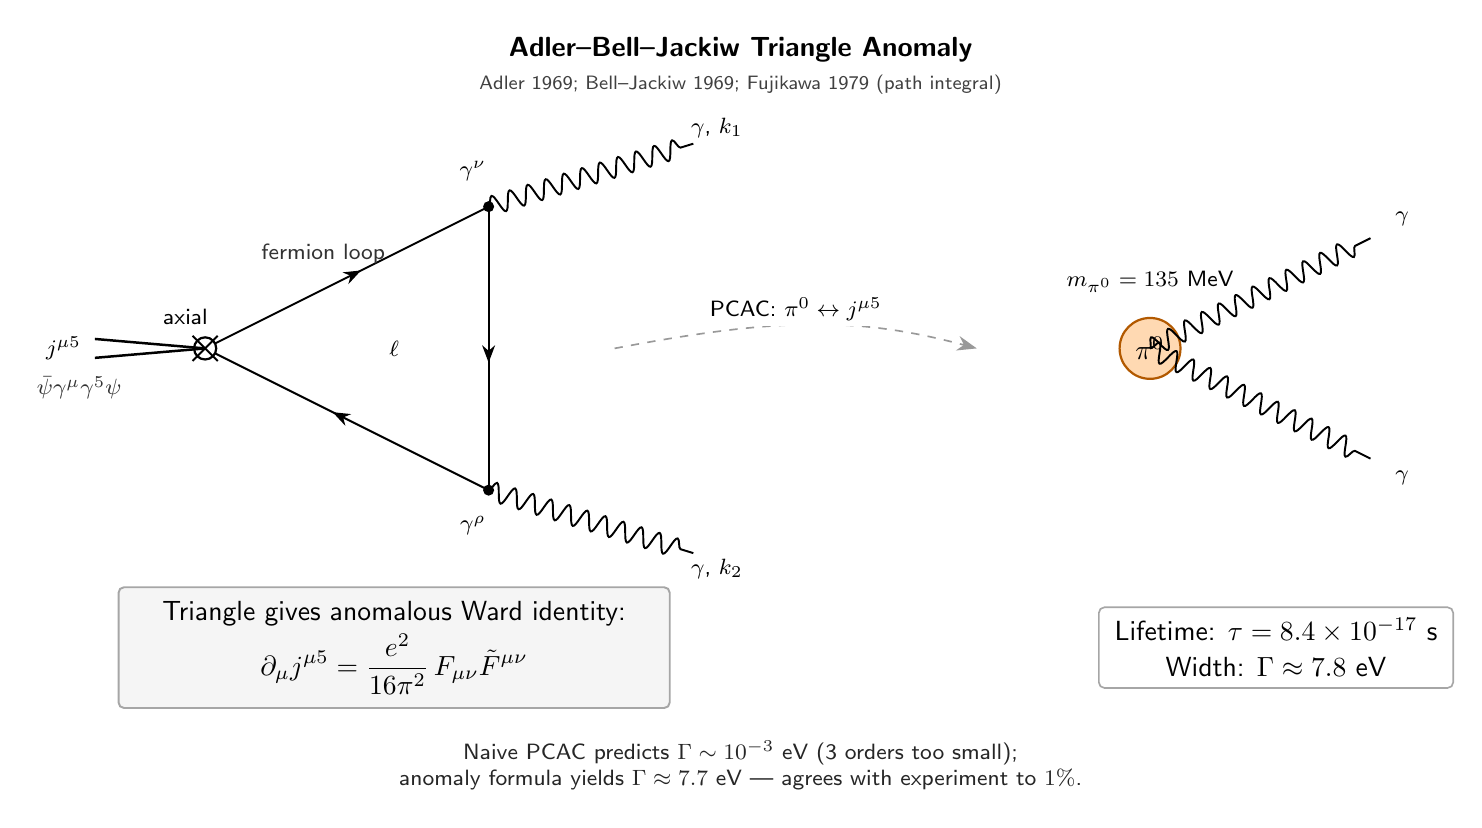
\begin{tikzpicture}[
    font=\sffamily,
    >={Stealth[length=2.5mm]},
    fermion/.style={postaction={decorate}, decoration={markings, mark=at position 0.55 with {\arrow{Stealth[length=2.2mm]}}}, line width=0.7pt, draw=black},
    photon/.style={decorate, decoration={snake, amplitude=1.2mm, segment length=2.4mm, post length=1.2mm}, line width=0.7pt, draw=black},
    dashedline/.style={dashed, line width=0.6pt, draw=gray!80, ->},
    vertex/.style={circle, fill=black, inner sep=0pt, minimum size=4pt},
    axialvertex/.style={circle, draw=black, line width=0.8pt, fill=white, inner sep=0pt, minimum size=8pt},
    pizero/.style={circle, draw=orange!70!black, line width=0.8pt, fill=orange!30, inner sep=0pt, minimum size=22pt},
    eqbox/.style={rectangle, draw=gray!70, line width=0.7pt, rounded corners=2pt, fill=gray!8, minimum width=7.0cm, minimum height=1.0cm, align=center, inner sep=5pt},
    infobox/.style={rectangle, draw=gray!70, line width=0.6pt, rounded corners=2pt, fill=white, minimum width=4.5cm, minimum height=0.8cm, align=center, inner sep=4pt},
    label/.style={font=\footnotesize\sffamily},
    titlestyle/.style={font=\bfseries\sffamily}
]

% =============== Title at top ==================
\node[titlestyle] at (0, 7.0) {Adler--Bell--Jackiw Triangle Anomaly};
\node[font=\scriptsize\sffamily, text=gray!50!black] at (0, 6.55) {Adler 1969; Bell--Jackiw 1969; Fujikawa 1979 (path integral)};

% =============== LEFT: Triangle Feynman Diagram ==================
% Triangle vertices (equilateral-ish)
\coordinate (V1) at (-6.8, 3.2);   % left vertex (axial)
\coordinate (V2) at (-3.2, 5.0);   % top-right vertex (photon 1)
\coordinate (V3) at (-3.2, 1.4);   % bottom-right vertex (photon 2)

% Fermion lines forming the triangle (with arrows showing loop direction)
\draw[fermion] (V1) -- (V2);
\draw[fermion] (V2) -- (V3);
\draw[fermion] (V3) -- (V1);

% Loop momentum label
\node[label] at (-4.4, 3.2) {$\ell$};
\node[label, text=gray!40!black] at (-5.3, 4.4) {fermion loop};

% Axial vertex: cross-marked circle
\node[axialvertex] (AV) at (V1) {};
\draw[line width=0.7pt] ($(V1)+(-0.16,-0.16)$) -- ($(V1)+(0.16,0.16)$);
\draw[line width=0.7pt] ($(V1)+(-0.16,0.16)$) -- ($(V1)+(0.16,-0.16)$);

% Axial current insertion (double-line in)
\draw[line width=0.9pt] (-8.2, 3.32) -- (V1);
\draw[line width=0.9pt] (-8.2, 3.08) -- ($(V1)+(0,-0.0)$);
\node[label] at (-8.6, 3.2) {$j^{\mu 5}$};
\node[label, text=gray!40!black] at (-8.4, 2.7) {$\bar\psi\gamma^\mu\gamma^5\psi$};

% Photon vertices
\node[vertex] at (V2) {};
\node[vertex] at (V3) {};

% Outgoing photons
\draw[photon] (V2) -- ++(2.6, 0.8);
\draw[photon] (V3) -- ++(2.6, -0.8);
\node[label] at (-0.3, 6.0) {$\gamma$, $k_1$};
\node[label] at (-0.3, 0.4) {$\gamma$, $k_2$};

% Vertex labels
\node[label] at (-3.4, 5.45) {$\gamma^\nu$};
\node[label] at (-3.4, 0.95) {$\gamma^\rho$};
\node[label] at (-7.05, 3.6) {axial};

% Anomaly equation box below left
\node[eqbox] at (-4.4, -0.6)
    {Triangle gives anomalous Ward identity:\\[2pt]
     $\displaystyle \partial_\mu j^{\mu 5} = \frac{e^2}{16\pi^2}\, F_{\mu\nu}\tilde F^{\mu\nu}$};

% =============== Connector: PCAC dashed arrow ==================
\draw[dashedline] (-1.6, 3.2) .. controls (0.5, 3.6) and (1.5, 3.6) .. (3.0, 3.2);
\node[label, fill=white, inner sep=2pt] at (0.7, 3.7) {PCAC: $\pi^0 \leftrightarrow j^{\mu 5}$};

% =============== RIGHT: Physical pi0 -> gamma gamma ==================
\coordinate (PI) at (5.2, 3.2);

% pi0 disk
\node[pizero] (PIDISK) at (PI) {};
\node[font=\bfseries] at (PI) {$\pi^0$};

% Outgoing photons from pi0
\draw[photon] (PI) -- ++(2.8, 1.4);
\draw[photon] (PI) -- ++(2.8, -1.4);
\node[label] at (8.4, 4.85) {$\gamma$};
\node[label] at (8.4, 1.55) {$\gamma$};

% pi0 mass label
\node[label] at (5.2, 4.05) {$m_{\pi^0} = 135$ MeV};

% Lifetime / width box below right
\node[infobox] at (6.8, -0.6)
    {Lifetime: $\tau = 8.4 \times 10^{-17}$ s\\[1pt]
     Width: $\Gamma \approx 7.8$ eV};

% =============== Bottom comparison note ==================
\node[font=\footnotesize\sffamily, text=gray!30!black, align=center] at (0, -2.1)
    {Naive PCAC predicts $\Gamma \sim 10^{-3}$ eV (3 orders too small);\\
     anomaly formula yields $\Gamma \approx 7.7$ eV --- agrees with experiment to $1\%$.};

\end{tikzpicture}
\end{document}
